\documentclass[tt1]{penoverslag}

%%% PACKAGES
\usepackage{lipsum}
\usepackage{gensymb}
\usepackage [dutch] {babel}
\usepackage{graphicx}
\usepackage{amsmath}
\usepackage{listings}
\usepackage{subcaption}
\usepackage{lscape}
\usepackage[absolute]{textpos}
  \setlength{\TPHorizModule}{1cm}
  \setlength{\TPVertModule}{1cm}


\begin{document}

\team{Zilver} % teamkleur
\members{Sam Gielis\\
         Sophie Marien\\
         Toon Nolten\\
         Nele Rober\\
         Gerlinde Van Roey\\
         Maxim Van Mechelen} % teamleden

\maketitlepage

\begin{abstract}
Het P\&O-project heeft als doel vier autonome robots \textit{Team Treasure Trek} te laten spelen. De robots moeten hierbij in een onbekend doolhof op zoek naar een bepaald voorwerp. Elke robot krijgt zijn eigen voorwerp toegewezen. Wanneer een robot zijn voorwerp gevonden heeft, komt hij te weten met welke robot hij moet samenwerken. Elk duo moeten hun voorwerpen bij elkaar brengen. Het duo dat hier eerst in slaagt, wint. Dit verslag beschrijft de invulling die team Zilver aan het project gaf.\\

De robot is voorzien van een lichtsensor, een infraroodsensor en een ultrasone sensor. De twee laatste sensoren staan vast gemonteerd en kunnen niet onafhankelijk van de robot bewegen. De lichtsensor kan wegklappen opdat de robot over een wip kan rijden. Verder is de robot voorzien van een soort schep met klittenband waarmee hij het voorwerp, dat ook voorzien is van klittenband, kan oprapen. Dit gebeurt door het voorwerp te klemmen tussen de muur en de robot zodat het in de schep valt.\\

De robot kan een doolhof verkennen en hiervan een map van bijhouden. Wanneer een tegel gevonden wordt die mogelijk een voorwerp bevat, zal deze tegel eerst nagekeken worden alvorens de robot verder het doolhof verkend. Via RabbitMQ \cite{RabbitMQ} kunnen de robots en simulators met elkaar communiceren. Zo kunnen de duo's een plaats afspreken om elkaar te ontmoeten.\\

Een computerprogramma simuleert de werking van robots. Deze simulator kan vier robots tegelijk simuleren of kan in hybride vorm gebruikt worden (waarbij \'e\'en fysieke en drie virtuele robots gebruikt worden). De gesimuleerde robots gedragen zich dan volledig analoog aan de fysieke robot.
\end{abstract}

\setcounter{tocdepth}{2}
\tableofcontents
%figuur robot
\begin{figure}[!hb]
\begin{textblock}{38}(4.5,15.5)
    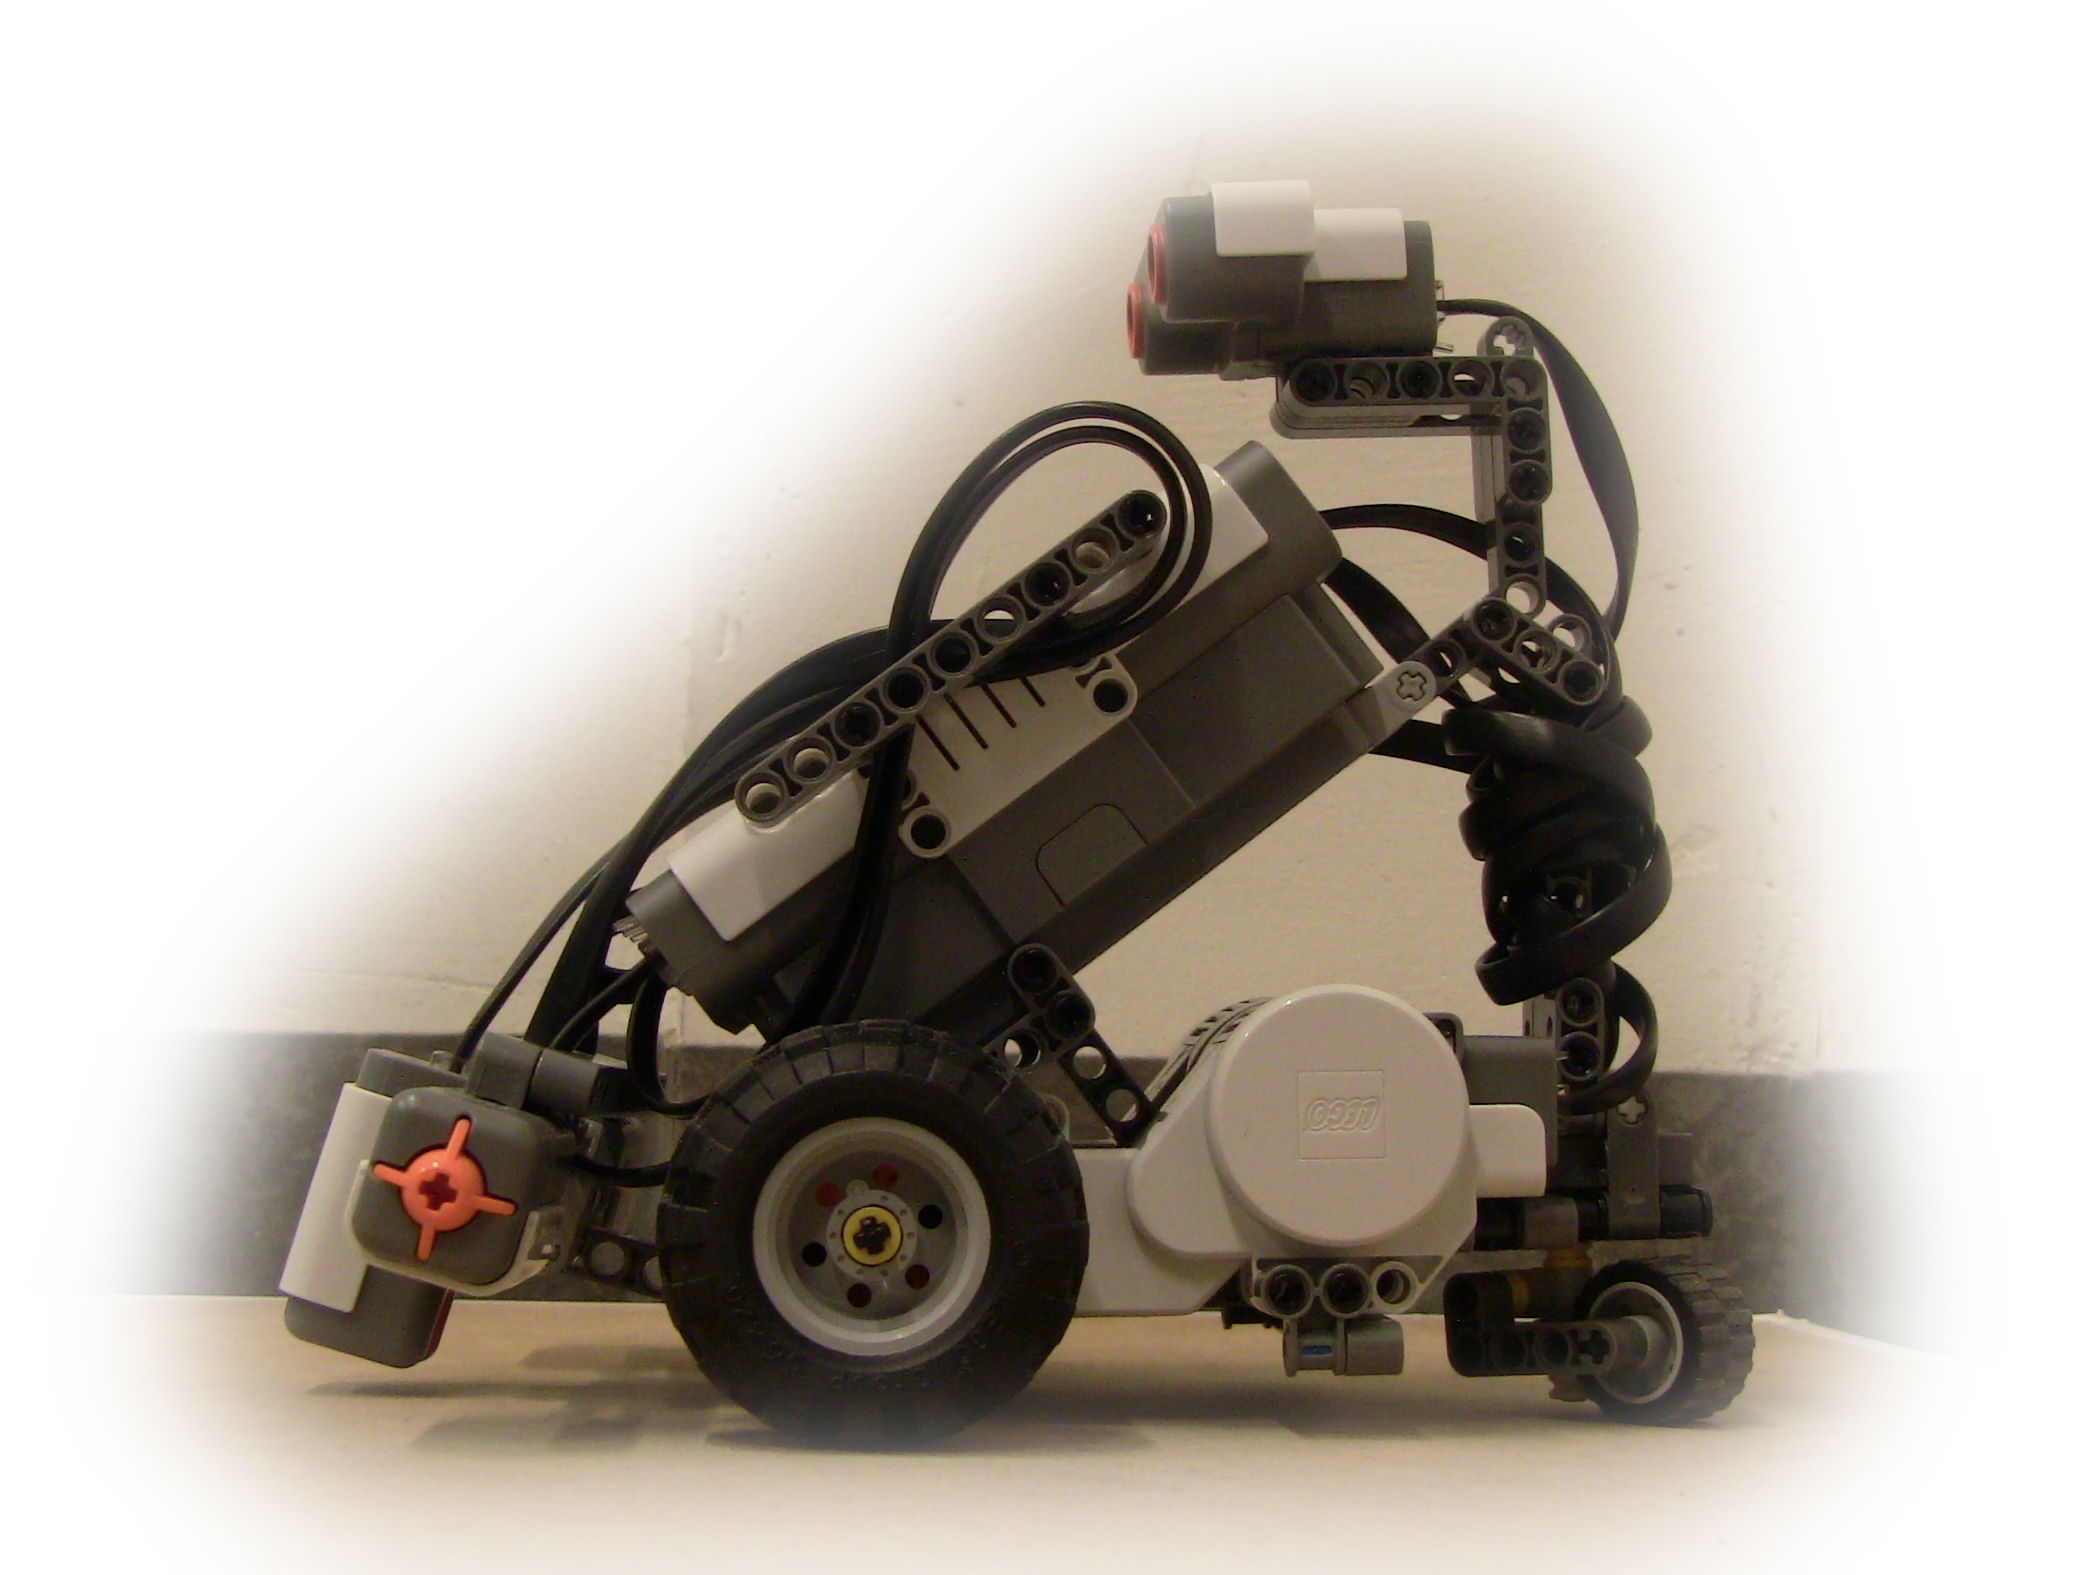
\includegraphics[width=0.5\textwidth]{robotFP}
    \label{fig:robotFP2}
\end{textblock}
\end{figure}

\newpage


% == INLEIDING == %
\section{Inleiding} % 4 ok
\label{ssec:inl}
In het kader van het vak `Probleemoplossen en Ontwerpen: computerwetenschappen' wordt gewerkt rond autonome intelligente robots. Verschillende teams bouwen en programmeren een robot met behulp van LEGO Mindstorms \cite{mindstorms}. Deze robot moet uiteindelijk samen met drie andere robots volledig autonoom \textit{Team Treasure Trek} kunnen spelen.\\

De eerste demonstratie bestaat erin de robot te laten rondrijden in een doolhof. De robot is in staat zijn voorwerp te zoeken en op te pikken terwijl de drie overige robots gesimuleerd worden. Bij het oppikken moet de robot dit laten weten aan zijn teamgenoot. Het is ook mogelijk met vier virtuele robots te werken. De virtuele robots communiceren met elkaar via RabbitMQ.\\


\section{Bouw robot}
\label{ssec:bouwrob}
LEGO Mindstorms \cite{mindstorms} biedt een bouwpakket voor een robot aan. Een NXT-microcomputer laat toe de robot te programmeren. Met behulp van leJOS \cite{leJOS} kan dit in Java.


\subsection{Fysieke bouw}
\label{ssec:fysb}

De fysieke bouw van de robot is grotendeels gebaseerd op die van het eerste semester. Enkele aanpassingen waren echter nodig om de robot geschikt te maken voor de nieuwe opdracht. De robot moet in staat zijn een voorwerp, met name een wc-rolletje, op te nemen. Verder bevat de opdracht enkele aspecten die extra sensoren impliceren: het detecteren van andere robots, het detecteren van de wip, vaststellen of het voorwerp daadwerkelijk is opgepakt,...\\
 
Op vlak van sensoren zijn twee aspecten verandert ten opzichte van het eerste semester. De druksensoren aan weerszijde van de lichtsensor zijn weggehaald. Deze hadden als doel te detecteren wanneer er tegen een muur werd gebotst tijdens het witte-lijnalgoritme. Ze zijn echter nooit ge\"implementeerd en bleken ook niet nodig te zijn.

Een infraroodsensor werd gemonteerd bovenop de robot. Deze infraroodsensor kan infraroodlicht detecteren. Er is een bal beschikbaar die dit infraroodlicht uitzendt. Wanneer deze bal onder een wip geplaatst wordt\footnote{De Scheidsrechtercommissie heeft nog niet besloten of de al hiervoor gebruikt zal worden.}, kan de robot makkelijk detecteren of de wip omhoog staat (en dus niet toegankelijk is) of omlaag. In dat tweede geval blokkeert de wip immers al het licht en detecteert de sensor niets.\\

Verschillende opstellingen zijn mogelijk om het voorwerp mee te nemen. Er moet rekening gehouden worden met de beperking van bewegingsvrijheid die het voorwerp teweeg kan brengen. Het is mogelijk het voorwerp over de grond te laten slepen, maar dit zorgt voor extra wrijving en verhoogt de kans dat het voorwerp losgeraakt. Bovendien moet de robot een wip kunnen passeren, ook wanneer hij het voorwerp bij zich heeft. 
 
Aanvankelijk werd gekozen een schep achteraan de robot te monteren, gebruik makend van een extra motor om het voorwerp `op te scheppen' (zie figuur \ref{fig:robotBouw}). Dit geeft als voordeel dat de wip zonder probleem te gepasseerd kan worden en dat het voorwerp stevig vast zit. De robot krijgt dan echter een te grote lengte waardoor hij onmogelijk kan omkeren zonder tegen een muur aan te botsen. Deze opstelling kon daarom niet behouden worden.

De robot heeft een schep vooraan. De schep is opgebouwd uit een deel van een wc-rol. Dit is immers de ideale vorm om het voorwerp, het wc-rolletje, op te nemen. De schep is, net zoals het voorwerp, voorzien van een strook klittenband (nog niet op de foto). Dit biedt extra zekerheid dat het voorwerp niet verloren geraakt. Figuur \ref{fig:robotBouw} toont een gedetailleerd zicht op de schep en het voorwerp.\\

Net zoals vorig semester zijn de ultrasone- en de infraroodsensor vast gemonteerd op de robot. De lichtsensor~-~en de schep die hieraan vast hangt~-~kunnen echter bewegen ten opzichte van de robot. Dit gebeurt met behulp van een scharnier, er werd geen extra motor gebruikt. Dit is nodig om over een wip te kunnen rijden. Het scharnier zorgt ervoor dat de lichtsensor wegklapt bij contact met de wip en later door de zwaartekracht weer terug op zijn plaats klapt. Zo zit de lichtsensor niet in de weg.

% figuren robot, oud en nieuw
\begin{figure}
\centering
	\begin{subfigure}[h]{0.45\textwidth}
	\centering
		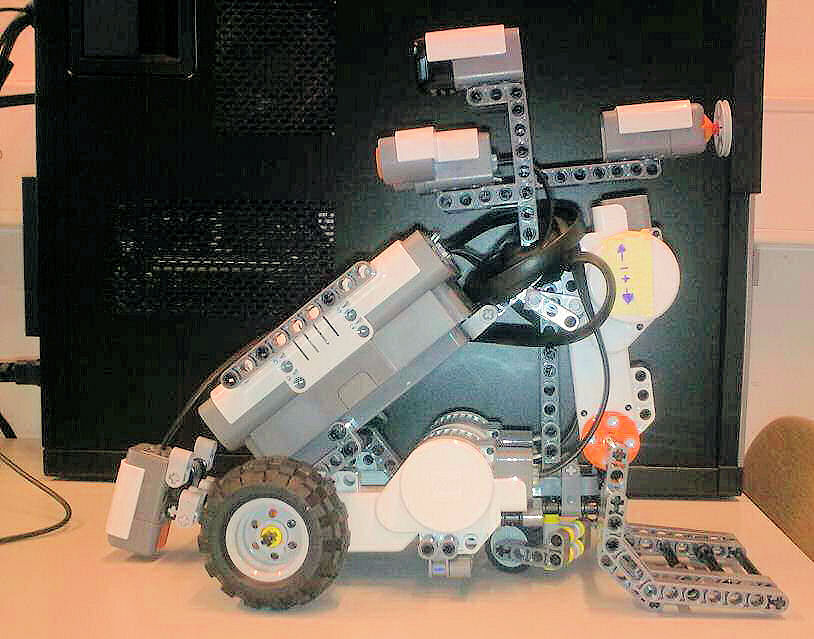
\includegraphics[width=\textwidth]{robotSchepOud}
		\caption{schep achteraan}
	\end{subfigure}%
	\begin{subfigure}[h]{0.47\textwidth}
		\centering
		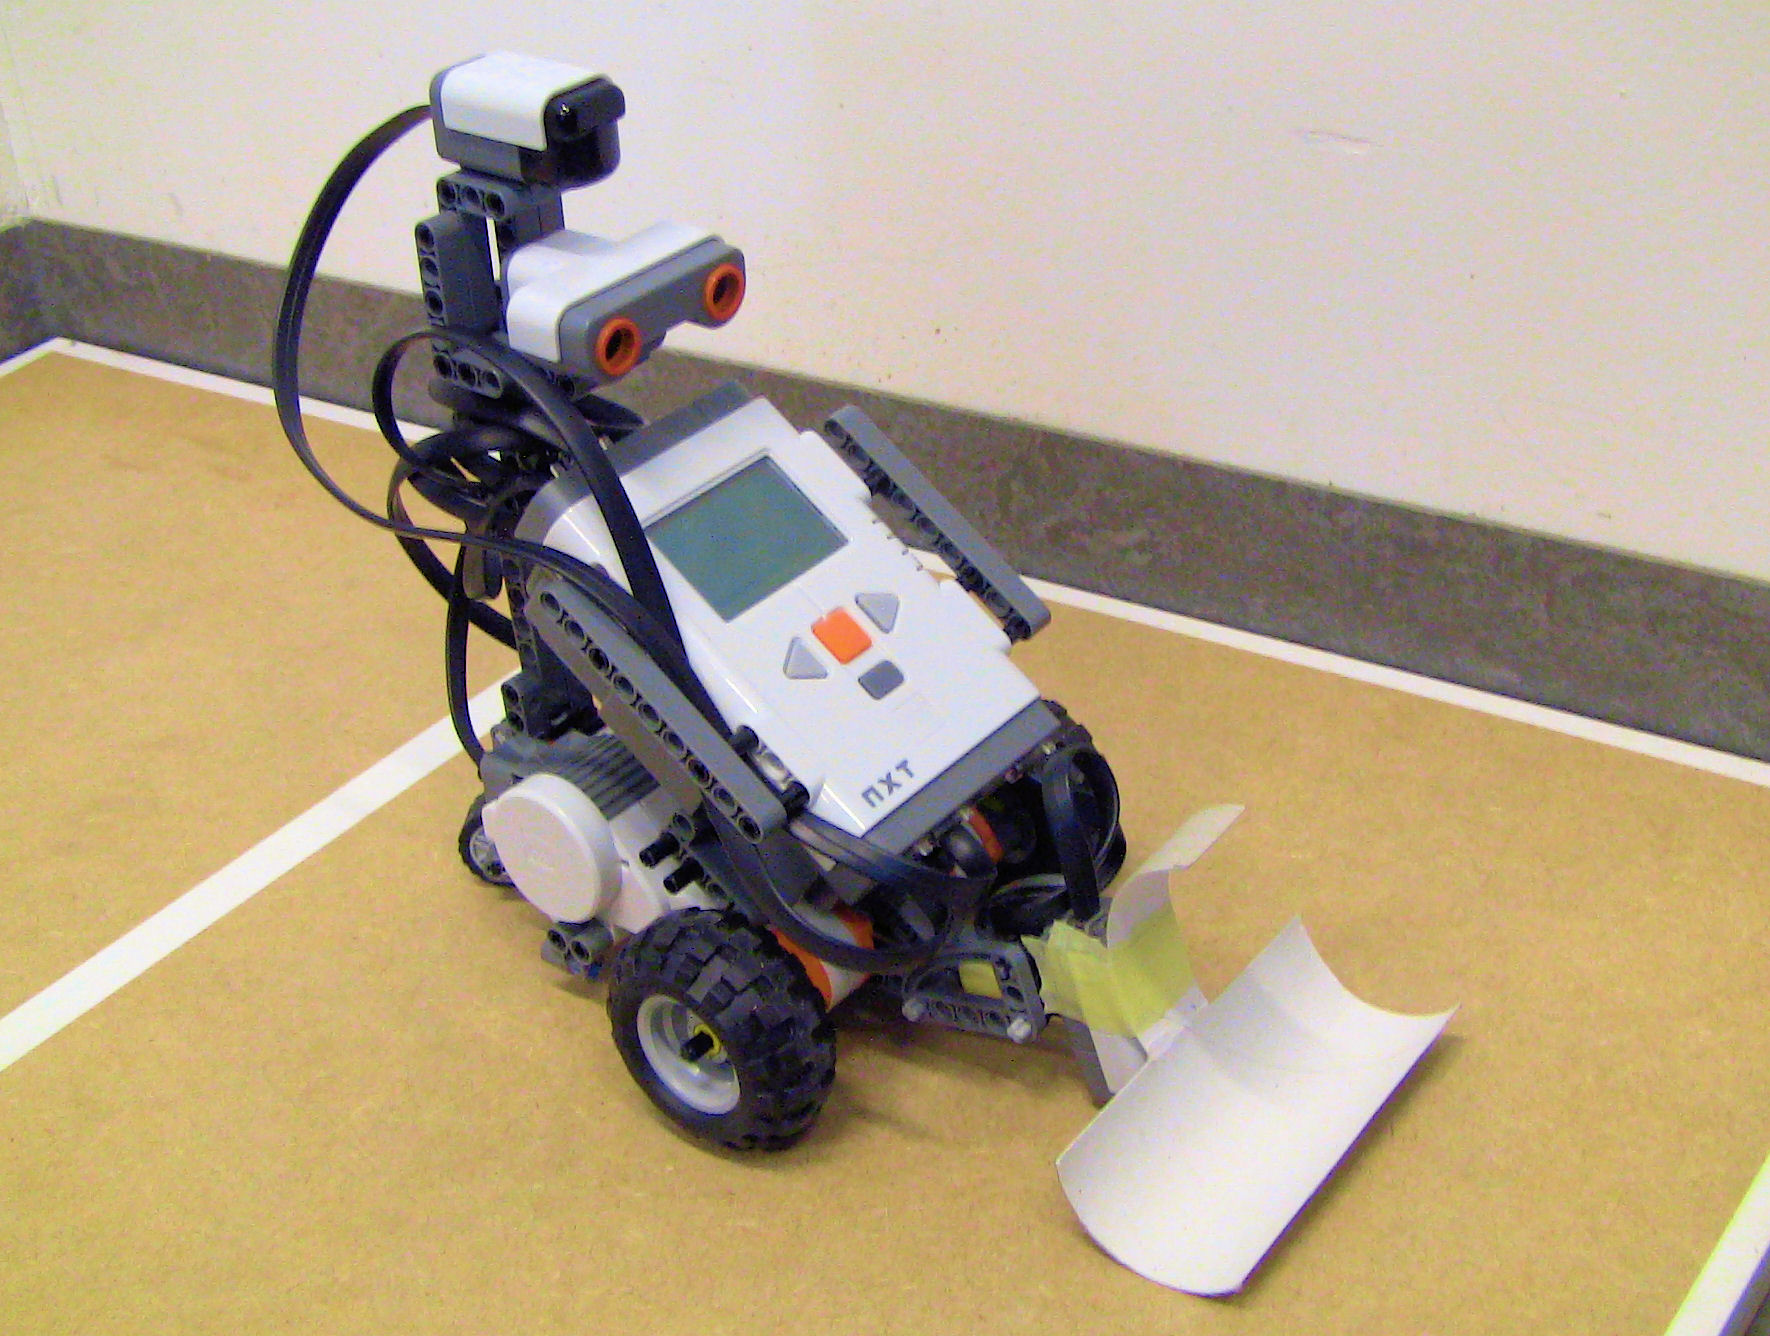
\includegraphics[width=\textwidth]{robotSchepNieuw}
	\caption{schep vooraan}
\end{subfigure}
\caption{Bouw van de robot.}
\label{fig:robotBouw}
\end{figure}

% figuren detail schep
\begin{figure}
\centering
	\begin{subfigure}[h]{0.46\textwidth}
	\centering
		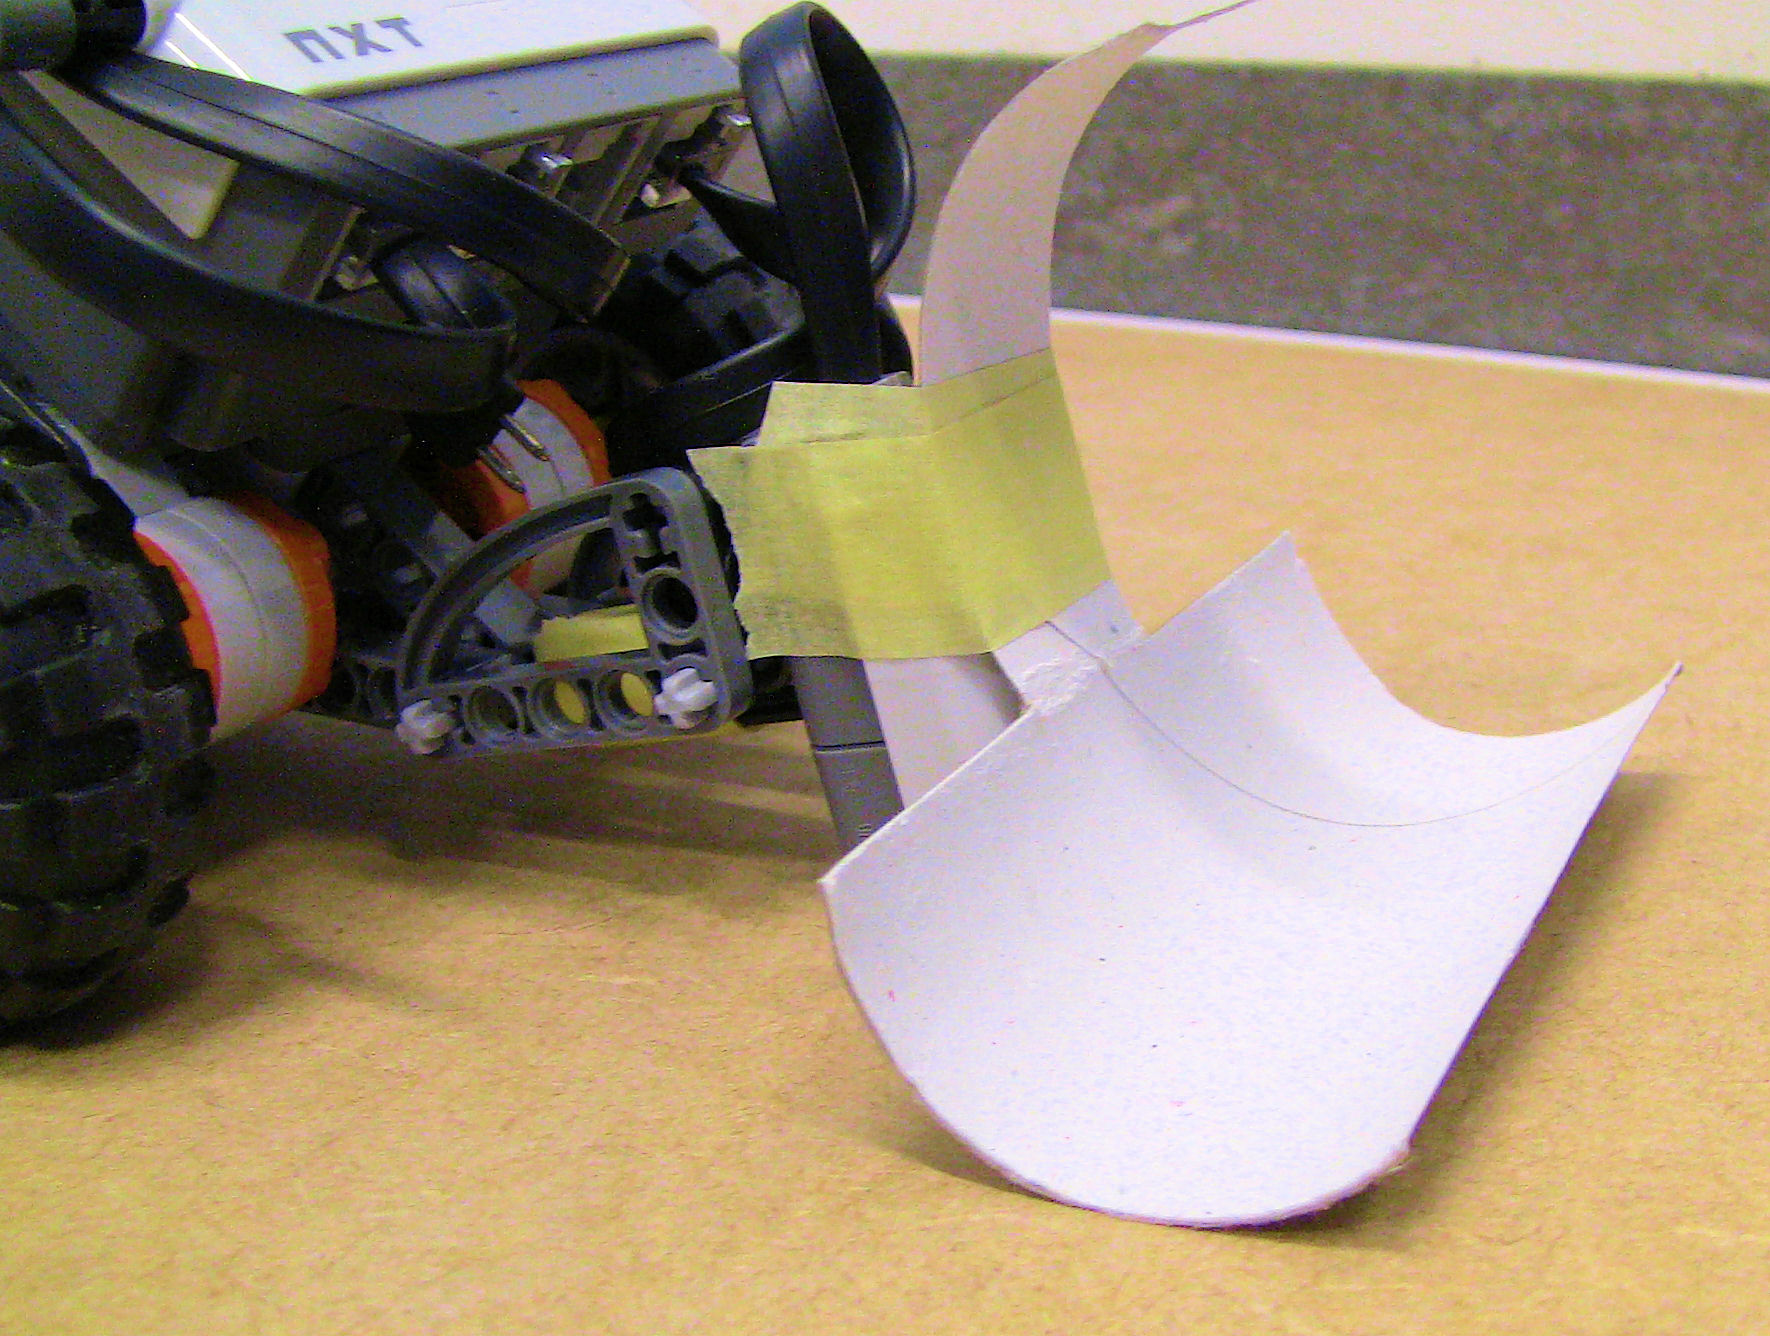
\includegraphics[width=\textwidth]{schepZonder}
	\end{subfigure}%
	\begin{subfigure}[h]{0.46\textwidth}
		\centering
		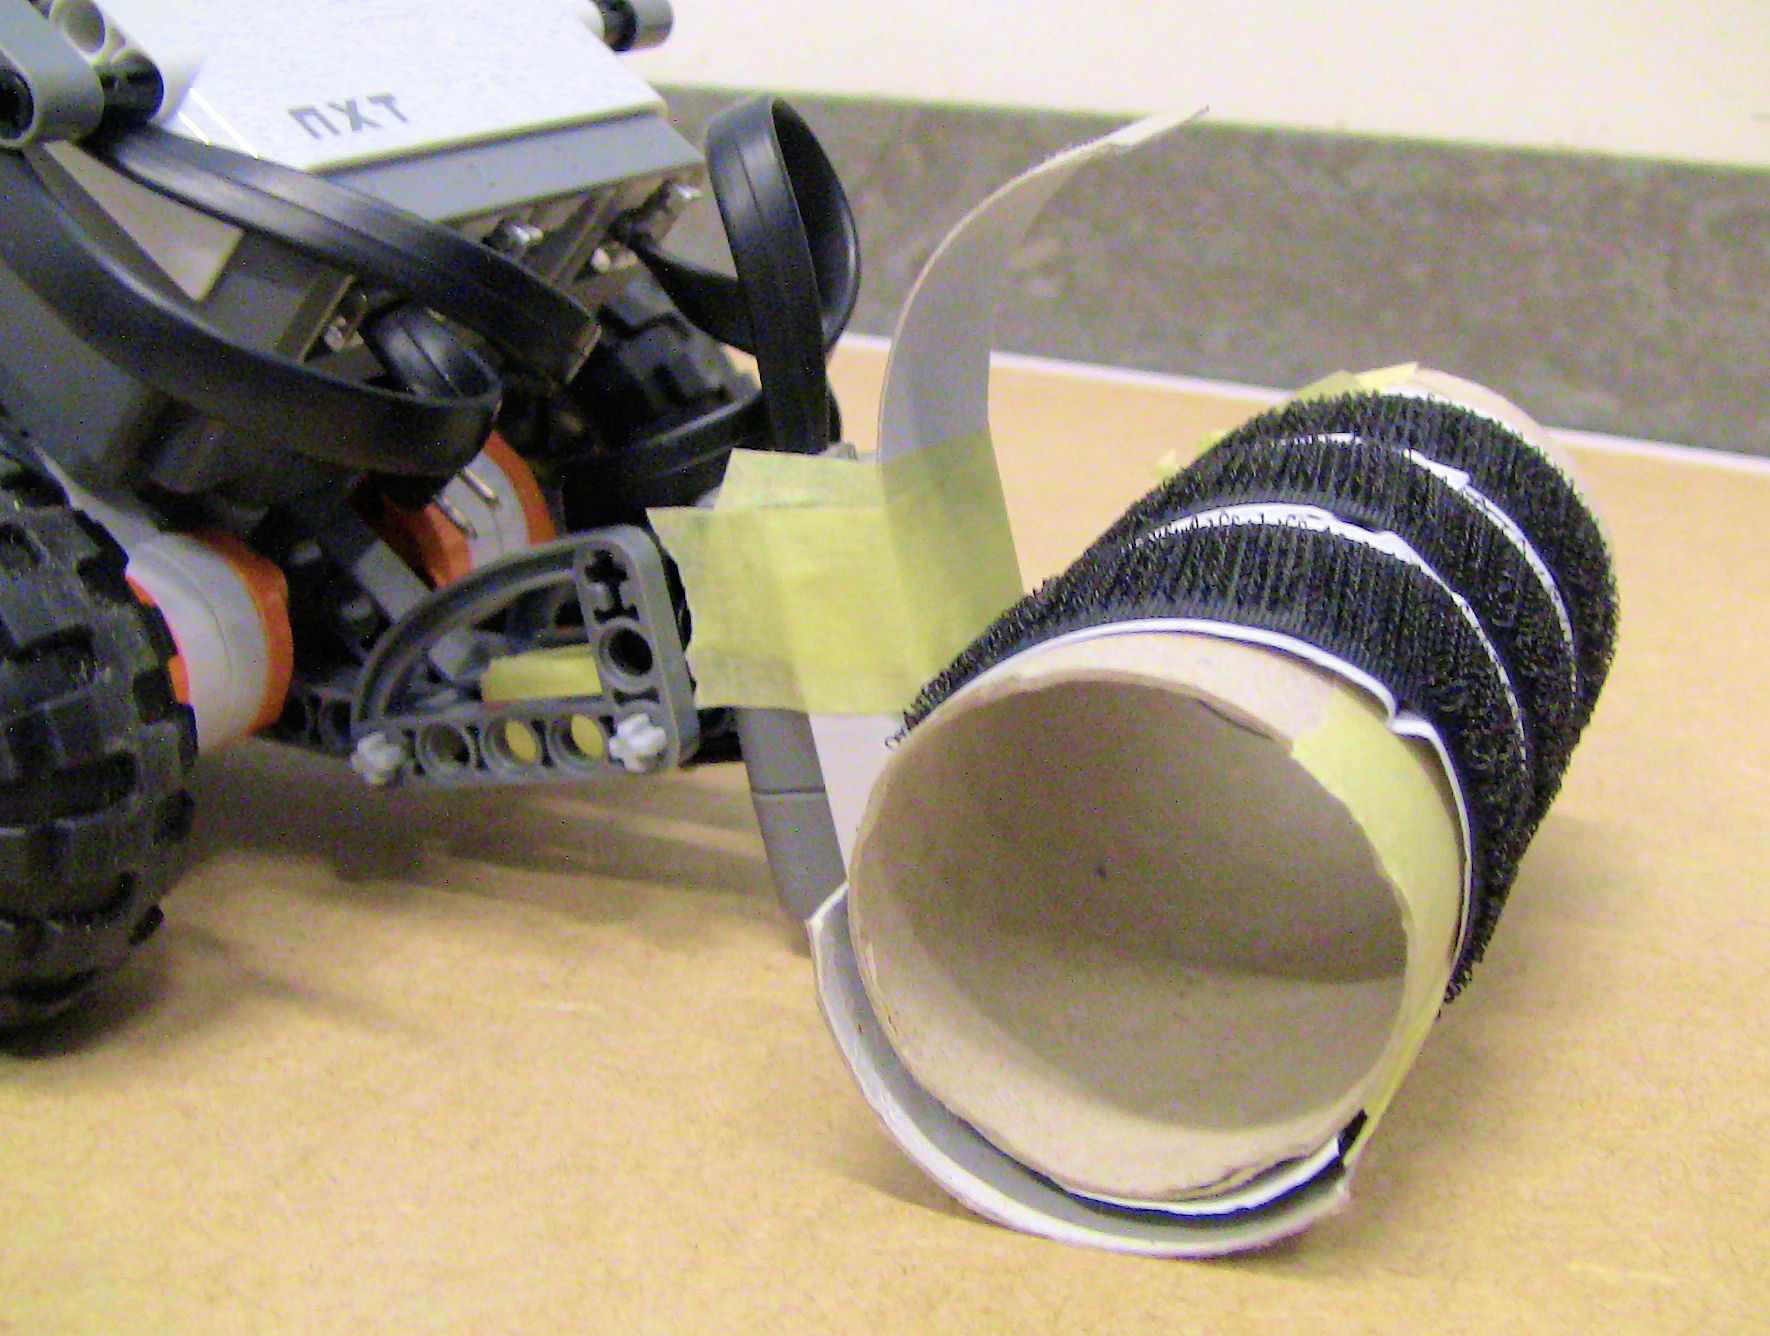
\includegraphics[width=\textwidth]{schepMet}
\end{subfigure}
\caption{Detail van de schep, met en zonder voorwerp.}
\label{fig:robotSchep}
\end{figure}


% == ALGORITMES == %
\section{Algoritmes}
Voor volgende algoritmes wordt verwezen naar het verslag van het eerste semester. Deze algoritmes worden dit semester zonder aanpassingen opnieuw gebruikt:
\begin{itemize}
	\item Rechtzetten op een witte lijn
	\item Centreren aan de hand van twee muren
	\item Lezen van een barcode
	\item Vinden van het kortste pad
\end{itemize}

% == zoeken van het voorwerp == %
\subsection{Zoeken van het voorwerp} %
\label{ssec:algoZoek}
Om het voorwerp te vinden moet de robot aanvankelijk het doolhof verkennen. De robot gebruikt hiervoor een implementatie van een geoptimaliseerd \textit{A*}. Deze optimalisaties worden beschreven in het verslag van het eerste semester.\\

Een extra optimalisatie geeft prioriteit aan het vinden van het voorwerp. Een voorwerp kan zich enkel bevinden op een `dead-end', voorafgegaan door een `straight' die een barcode bevat. Deze barcode identificeert het voorwerp. Wanneer een mogelijke voorwerp-locatie gevonden wordt, wordt zo snel mogelijk nagegaan of het om het juiste voorwerp gaat. In sommige gevallen is het niet mogelijk rechtstreeks naar de locatie te gaan omdat het doolhof daar nog niet verkend is. In dat geval wordt verder verkend in de richting van de locatie. De `dead-end' zelf hoeft niet bezocht te worden wanneer uit de barcode blijkt dat het niet om het juiste voorwerp gaat, zodat optimalisatie E nog steeds geldt.\\

Nadat het voorwerp gevonden is, probeert de robot zijn teamgenoot te contacteren. Indien de teamgenoot zijn voorwerp nog niet heeft of wanneer de mappen van beide robots nog niet combineerbaar zijn, gaat de robot verder met het verkennen van het doolhof. Hierbij wordt nog steeds prioriteit gegeven aan voorwerp-locaties. Deze bevatten immers unieke barcodes die het later makkelijker maken de mappen te combineren.

Als alternatief kan de robot zich naar het voorwerp van de teamgenoot begeven om daar op hem te wachten (niet te dicht bij om niet in de weg te staan). Deze extra optie wordt voorlopig nog niet ge\"implementeerd omdat nog niet duidelijk is in welke gevallen de strategie het best werkt.

% nog niet voor deze demo!
%\subsection*{Algoritme om zo snel mogelijk naar de andere robot te gaan}
%Hierbij dachten we aan het kortste-pad-algoritme. Dit zal wel nog aangepast moeten worden aan zowel draaien als vooruit rijden (draaien was nog niet in rekening gebracht).\\ Er moet ook nog rekening gehouden worden als de andere robot zou wegrijden. De robot mag hierdoor niet in een loop terechtkomen. Er zou moeten gecommuniceerd worden wie naar wie toerijdt, of dat er naar een gezamenlijke tegel moet gereden worden. \\
%Als de andere robot zou wegrijden zou er een afstand kunnen bijgehouden worden die dan opnieuw berekent wordt als de afstand niet kleiner wordt.

% == SOFTWARE == %
\section{Software}
\label{secc:softw}

Bij het aanvatten van het 2e P\&O-seizoen bleek dat het project qua code toch niet al te eenduidig en leesbaar was.
Het project is dan ook grondig herbouwd en gerefactord, zoals de aandachtige lezer die zowel dit als vorig verslag heeft gelezen, zal opmerken.\\
De software bestaat uit twee delen: een project dat op de NXT van de robot loopt (sectie \ref{ssec:Robot}) en een project dat op de computer loopt (sectie \ref{ssec:Sdesign}). Alles wordt aangestuurd via de \textit{Graphical User Interface (GUI)} (sectie \ref{ssec:GUI}). Deze laat toe de robot te besturen en de reacties van de robot weer te geven. Robots kunnen met elkaar communiceren via RabbitMQ (sectie \ref{ssec:RabbMQ}). Via de GUI kunnen ook een virtuele robots aangestuurd worden: de simulators (sectie \ref{ssec:Sim}).\\

Voor volgende secties wordt verwezen naar het verslag van het eerste semester. Deze implementaties en ontwerpen werden zonder aanpassingen opnieuw gebruikt:

\begin{itemize}
\item Commando's doorgeven
\item Bluetooth
\item Robot
\item Mappen van een doolhof
\end{itemize}

% -- Ontwerp -- %
\subsection{Ontwerp van het computerproject}
\label{ssec:Sdesign}
Een overzicht van het ontwerp wordt weergegeven in de klassendiagramma van figuur \ref{fig:klasdia}.\\

De Main-methode bevindt zich in de GUI-klasse. Deze maakt een \textit{SimulatorPanel}-object aan. Dit is een overkoepelend panel waarin meerdere \textit{Viewports} zitten. Een \textit{OverallViewport} geeft de volledige doolhof en alle robots erin weer. Dit kan uiteraard enkel wanneer een gekende virtuele doolhof gebruikt wordt. Een \textit{UnitViewport} geeft de wereld van \'e\'en robot (eventueel gesimuleerd) weer: de sensorwaarden en de muren die hij reeds ontdekt heeft. Dit is enkel mogelijk wanneer deze robot zijn informatie doorgeeft aan de \textit{Viewport}. Een wereld waarvan niets geweten is, kan niet worden weergegeven. Dit is het geval voor robots van andere teams, met uitzondering van de teamgenoot. Deze stuurt zijn map door, maar niet zijn sensorwaarden en wordt gerepresenteerd door een \textit{DummyViewPort}. Het aantal \textit{Viewports} hangt af van het aantal gekende werelden. Deze verdeling wordt weergegeven in tabel \ref{tab:aantViewports}.\\

Een \textit{DummyViewport} zal aanvankelijk niet worden weergeven. Deze \textit{Viewport} geeft de wereld van de teamgenoot weer. Wie deze teamgenoot is, wordt echter pas bekend wanneer beide leden van het team hun voorwerp gevonden hebben. Op dat moment zal het \textit{DummyViewport} verschijnen.\\

% figuren klassendiagramma
\begin{landscape}
\begin{figure}
\centering
	\begin{subfigure}{0.60\textwidth}
	\centering
		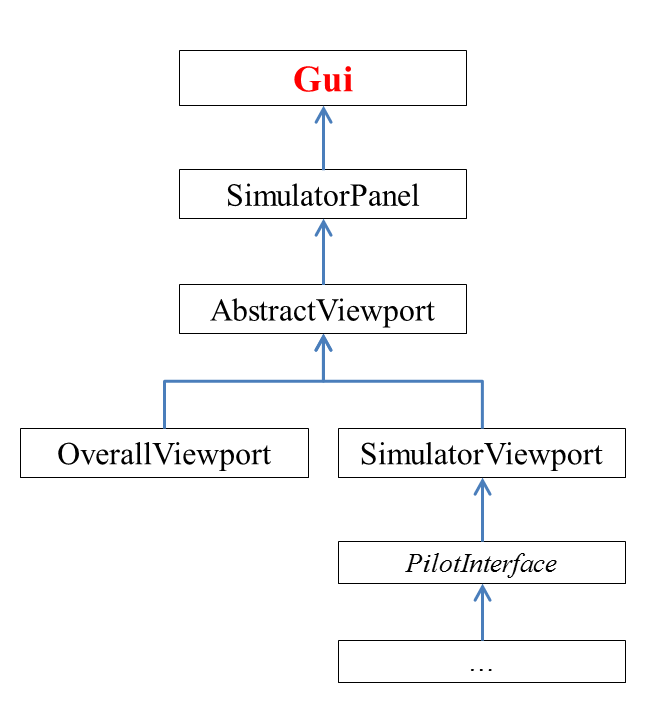
\includegraphics[width=\textwidth]{KlasGUI}
		\caption{GUI, SimulatorPanel en Viewports}
	\end{subfigure}%
	\begin{subfigure}{0.5\textwidth}
		\centering
		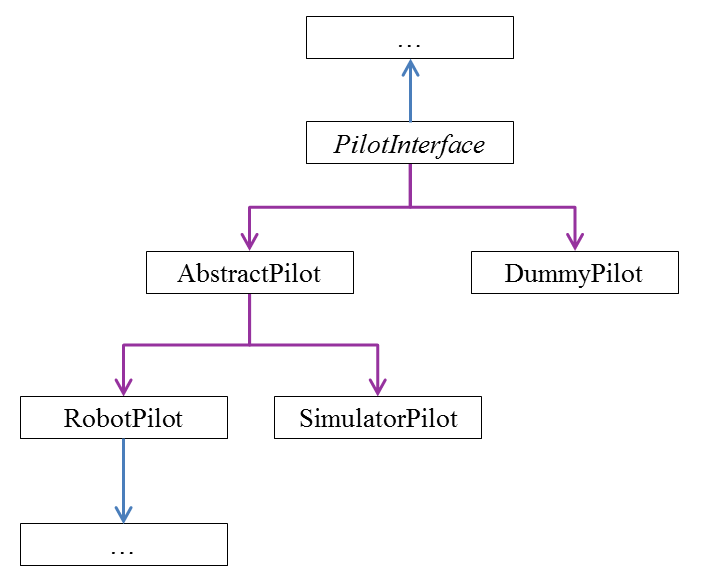
\includegraphics[width=\textwidth]{KlasPilot}
	\caption{Pilots}
\end{subfigure}%
\begin{subfigure}{0.45\textwidth}
		\centering
		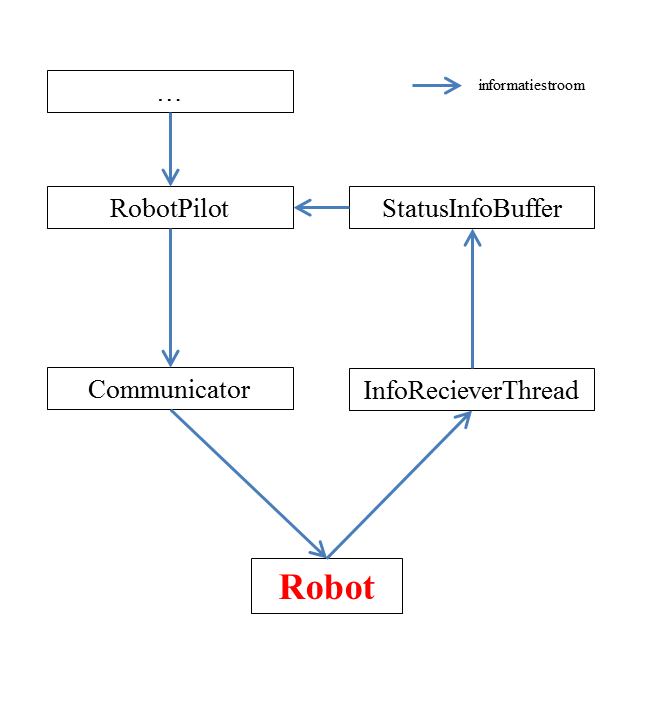
\includegraphics[width=\textwidth]{KlasRobot}
	\caption{Robot}
\end{subfigure}
\caption[Klassendiagramma]{Klassendiagramma (paarse pijlen wijzen op overerving of implementatie, blauwe op een informatiestroom)}
\label{fig:klasDia}
\end{figure}
\end{landscape}

% tabel #viewports
\begin{table}
\begin{center}
    \begin{tabular}{ c | c | c || c | c | c }
    wij & wij & anderen & aantal & aantal & aantal\\
    fysiek & gesimuleerd & fysiek/gesimuleerd & OveralViewports & UnitViewports & DummyViewports\\ \hline \hline
    1 & 3 & 0 & 1 & 4 & 0\\
    0 & 4 & 0 & 1 & 4 & 0\\
    1 & 0 & 3 & 0 & 1 & 1\\
    0 & 1 & 3 & 0 & 1 & 1\\
    \end{tabular}
    \caption{Overzicht aantal OveralViewports en aantal UnitViewports}
    \label{tab:aantViewPorts}
\end{center}
\end{table}

Elke \textit{Viewport} maakt een eigen \textit{Pilot} aan. Er zijn verschillende soorten \textit{Pilots} die elk een implementatie van \textit{PilotInterface} zijn. De keuze van \textit{Pilot} hangt af van het type robot. Een robot waarvan de wereld niet kan worden voorgesteld, heeft een \textit{DummyPilot}. Deze bevat enkel `getters', want deze robot kan niet worden aangestuurd. Een robot die gesimuleerd wordt, heeft een \textit{SimulatorPilot}. Deze berekent zelf zijn sensorwaarden op basis van een virtuele doolhof. Een fysieke robot krijgt een \textit{RobotPilot} die via de \textit{Communicator} in verbinding staat met de fysieke robot. Deze krijgt zijn sensorwaarden terug van de robot via de \textit{InfoReceiversThread} en de \textit{StatusInfoBuffer}. Deze \textit{Pilots} zijn de `hersenen' van deze robots/simulators. De \textit{Viewports} geven enkel weer wat de robots uitvoeren, zij berekenen en beslissen niets.

% -- GUI -- %
\subsection{Grafische User Interface}
\label{ssec:GUI}

% figuren GUI
\begin{figure}[hb]
\centering
	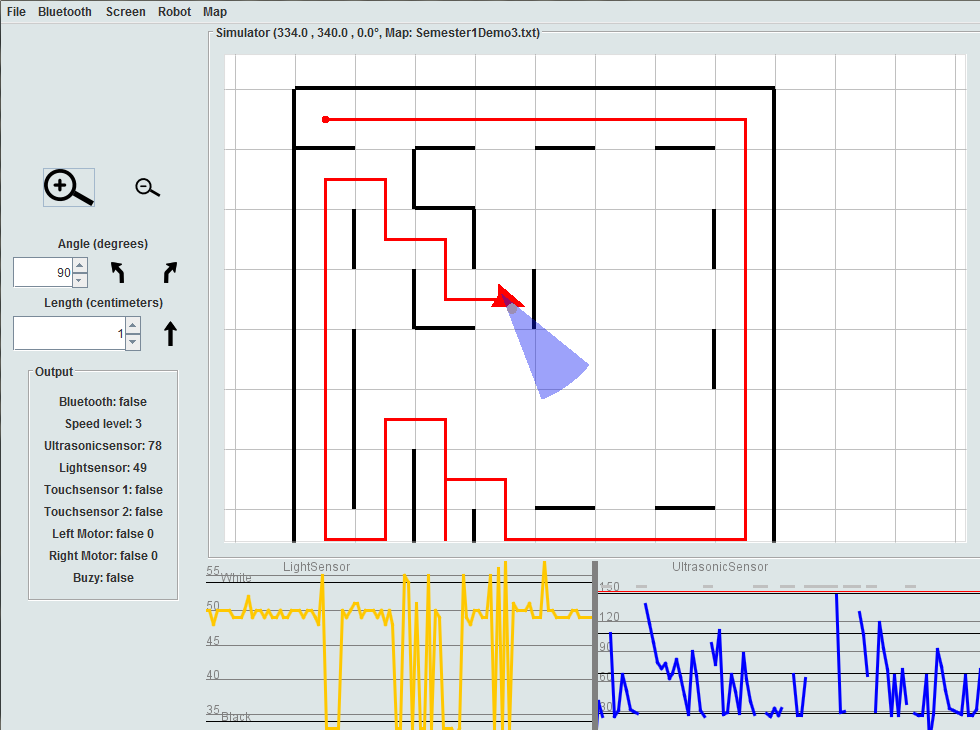
\includegraphics[width=0.8\textwidth]{GUI}
\caption{de Graphical User Interface}
\label{fig:GUI}
\end{figure}

De GUI zal er wat anders uitzien dan van vorig semester. Het moet nu immers mogelijk zijn de wereld van meerdere robots tegelijk weer te geven. Deze werelden verschillen van elkaar: zeker in het begin verkennen de verschillende robots een ander deel van het doolhof. Omdat zowel beginpositie als -ori\"entatie niet gekend zijn, is het niet mogelijk al deze werelden in \'e\'en paneel weer te geven. Het \textit{SimulatorPanel} wordt opgedeeld in verschillende \textit{Viewports}. Zoals uitgelegd in sectie \ref{ssec:Sdesign} hangt het aantal \textit{Viewports} af van de situatie.\\

Wanneer de robot een pad aflegt, tekent de \textit{UnitViewport} dit in het tekenpaneel als een rode lijn (herschaald: \'e\'en cm = \'e\'en pixel). De lijnen worden als lijnen opgeslagen in de \textit{UnitViewport}. Wanneer de robot een rechte weg aflegt, wordt het eindpunt van de gedefinieerde lijn steeds verlegt. Dit zorgt ervoor dat de weg die de robot aflegt continu bijgewerkt wordt. De huidige positie en de huidige ori\"entatie van de robot wordt weergegeven door een driehoek die draait met de ori\"entatie. Het bereik van de gesimuleerde ultrasone sensor wordt grafisch weergegeven door een blauwe boog. De lichtsensor wordt voorgesteld als een bol die van kleur verandert wanneer de ondergrond wijzigt. 
Een \textit{DummyViewport} geeft geen pad of sensorwaarden weer, enkel een map. De map-in-opbouw wordt weergegeven op basis van de map die de \textit{Pilot} opstelt.\\

Al deze \textit{Viewports} nemen plaats in, waardoor andere functionaliteiten van de GUI naar de achtergrond moeten verdwijnen. De sensorgrafieken, bijvoorbeeld, zullen nog beschikbaar zijn, maar worden enkel zichtbaar wanneer deze via een menu expliciet geopend worden. Zo kunnen ze nog steeds gebruikt worden voor testen.\\

De nieuwe GUI is nog niet volledig klaar, dus is een figuur van de GUI bijgevoegd zoals deze er in het eerste semester uit zag: figuur \ref{fig:GUI}.


% -- RabbitMQ -- %
\subsection{RabbitMQ}
\label{ssec:RabbMQ}
De implementatie van RabbitMQ \cite{RabbitMQ} is sterk gebaseerd op de demo die op Toledo werd geplaatst.\\

Elke \textit{AbstractPilot} moet kunnen interageren met een RabbitMQ-kanaal. De klasse \textit{MessageCenter} zorgt voor een RabbitMQ-interface die de pilots kunnen gebruiken. Het object verbindt met een server bij initialisatie. Enkele algemene parameters worden meegegeven: user name, password, port,... De belangrijkste methodes in de klasse zijn \textit{sendMessage()} en \textit{subscribeTo()} die respectievelijk het schrijven naar en monitoren van specifieke `exchanges' en `queues' toelaten. De methodes aanroepen heeft volgend effect:\\

\begin{description}
\item[subscribeTo(String monitorKey):] Een object van de klasse \textit{SubscribeMonitor} wordt aangemaakt. Deze \textit{SubscribeMonitor} luistert naar alle berichten op het kanaal van het \textit{MessageCenter} die met de gegeven string beginnen (de `Monitor Key'). Vervolgens stuurt het \textit{MessageCenter} al deze informatie naar de \textit{AbstractPilot} die de monitoring-aanvraag deed. Deze Pilot ontvangt vanaf dan alle berichten met het onderwerp waarvoor hij een aanvraag deed, maar van berichten met een ander onderwerp krijgt hij geen melding.
\item[sendMessage(String exchange, String routingKey, String message):] Dit bericht wordt naar de gespecifi\"eerde `exchange' gestuurd. Deze plaatst het bericht in alle `queues' die het onderwerp (gespecifi\"eerd door de routingKey) volgen. Op deze manier krijgen alle \textit{Pilots} die aanvraag deden voor het onderwerp, melding van het bericht.
\end{description}

% -- Simulator -- %
\subsection{Simulator}
\label{ssec:Sim}
De \textit{Simulator} bootst de werking van de robot virtueel na. Hij kan dezelfde commando's uitvoeren als de werkelijke robot en berekent sensorwaarden die een echte robot zou genereren wanneer deze zich in een soortgelijke situatie bevindt.\\

De \textit{SimulatorPilot} bepaalt de positie van de `robot' ten opzichte van het virtuele doolhof: hoe ver van de muur en op welke ondergrond. Tests op de echte robot in gelijkaardige situaties laten toe een waarde te simuleren die dicht aansluit bij de echte waarde. De \textit{SimulatorPilot} haalt zijn referenties uit de klasse \textit{SimulationSensorData} die meetresultaten van de echte robot bijhoudt. De sensorwaarden worden niet nauwkeurig gegenereerd: er werd ruis toegevoegd. De echte robot geeft immers ook geen exacte waarden.\\

De \textit{AbstractPilot} bepaalt hoe de gesimuleerde robot moet reageren in de gegeven situatie. De klasse bevat methodes als \textit{travel()} en \textit{rotate()}. Ook bouwt de \textit{AbstractPilot} een map op terwijl de robot zich voortbeweegt door het doolhof. De \textit{AbstractPilot} kan zowel de echte robot als een gesimuleerde robot aansturen. De \textit{AbstractPilots} zijn de hersenen van de robots.




% == BESLUIT == %
\section{Besluit}
De uiteindelijke bouw van de robot bestaat uit een infrarood sensor vanboven op de ultrasone sensor en een schepsysteem voor het voorwerp vooraan de robot. Op het schepsysteem is velcro aangebracht zodat het voorwerp stevig vastzit. De lichtsensor heeft een scharnier gekregen, zodat als de robot over een wip rijdt, de lichtsensor niet in de weg zit. \\

De GUI heeft vele verandering ondergaan ten opzichte van het vorige semester. Zo is het aangepast dat het nu ook de tegenstanders kan simuleren en de teamgenoot. Dit wordt gedaan via viewports.\\
Verder moest ook de communicatie geimplementeerd worden zodat de robot een bericht kon uitsturen dat het zijn voorwerp gevonden had. 
De robot communiceert met de andere robotten via RabbitMQ. Hiermee kan de robot afspraken maken met de andere robot en zo ook te weten komen wie zijn teamgenoot is.
 





\newpage
\bibliographystyle{siam}
\bibliography{biblio.bib}

\begin{thebibliography}{9}
\bibitem{mindstorms}
\textit{Lego Mindstorms}:  Een uitbreiding op de LEGO bouwstenen waarmee kleine, aanpasbare en programmeerbare robots gebouwd kunnen worden. Een centrale besturingsmodule (`the brick') kan geprogrammeerd worden met verschillende programmeertalen. In eerdere versies werd een RCX gebruikt voor de brick, nu wordt met NXT gewerkt. De brick kan enkele motoren aandrijven. Bovendien kunnen er verschillende sensoren, o.a. een ultrasone sensor en een lichtsensor, aangesloten worden.  \mbox{[www.lego.com]} \mbox{[http://en.wikipedia.org/wiki/Lego\textendash Mindstorms]}

\bibitem{leJOS}
\textit{leJOS}: Een kleine Java Virtuele Machine die toelaat de NXT-brick te programmeren. leJOS voorziet verschillende klassen die o.a. de motoren aansturen en een bluetoothverbinding opzetten.  \mbox{[http://lejos.sourceforge.net/]}

\bibitem{RabbitMQ}
\textit{RabbitMQ}: RabbitMQ is een communicatiesysteem dat het Advanced Message Queing Protocol (AMQP) implementeert. Door een kanaal op te zetten met een RabbitMQ-server is het mogelijk een bericht te plaatsen dat anderen kunnen lezen. De server heeft enkele `exchanges' die verdelen de berichten over `queues'. Die queues worden aangemaakt door de clients en luisteren elk naar een bepaald onderwerp. De exchange pushed dus berichten met een bepaald onderwerp naar de juiste queues.
\mbox{[http://en.wikipedia.org/wiki/RabbitMQ]}


\end{thebibliography}


\end{document}
